\chapter{Einleitung}

\section{Motivation}

In der Literatur findet man viele verschiedene Definitionen eins verteiltes Systems. Vieler dieser Definitionen unterschieden sich untereinander, so dass es schwerf\"{a}llt eine Definition zu finden, die als Alleinige als die Richtige gilt. Andrew Tanenbaum und Marten van Steen haben f\"{u}r die Beschreibung eins verteilten Systems die Folgende lockere Charakterisierung formuliert:

\cite{Tanenbaum} \textit{``Ein verteiltes System ist eine Menge voneinander unabh\"{a}ngiger Computer, die dem Benutzer wie ein einzelnes, koh\"{a}rentes System erscheinen''}

\begin{figure}[htbp]
	\centering
	\fbox{\includegraphics{images/verteiltes-system}}
	\caption{Ein verteiltes System bestehend aus 4 Computern}
	\label{fig:VerteiltesSystem}
\end{figure}

Demnach erscheint dem Benutzer ein aus mehreren Computern bestehendes verteiltes System wie ein System, welches lediglich aus einem einzigen Computer besteht. Der Benutzer muss sich nur mit dem lokalen vor ihm befindenden Computer auseinandersetzen (Abbildung \ref{fig:VerteiltesSystem}). Die Software des lokalen Computer stellt die reibungslose Kommunikation mit anderen Computern des verteilten Systems sicher und der Benutzer muss sich darum nicht selbst k\"{u}mmern.\\
\\
Hier betrachten wir ein verteiltes System von einer anderen Perspektive. Wir nehmen nicht die Sichtweise eines Endbenutzers ein, sondern wollen die grundlegenen Funktionsweisen, wie unabh\"{a}ngige Computer in einem verteilten System miteinander agieren, verstehen. Es sollen alle relevanten Ereignisse eines verteilten Systems sichtbar und verst\"{a}ndlich repr\"{a}sentiert werden.

Um dieses Ziel zu erreichen wurde ein Simulator entwickelt, der dies erm\"{o}glicht. Der Simulator wurde insbesondere f\"{u}r Lehr- und Lernzwecke entwickelt. Er inspiriert auch die Entwicklung eigener verteilter Systeme. 

\section{Grundlagen}

F\"{u}r das Verst\"{a}ndnis wie die Simulation von verteilten Systemen funktioniert, werden hier einige Grundbegriffe erl\"{a}utert. Eine Vertiefung findet erst in den nachfolgenden Kapiteln statt.

\subsubsection{Client/Server Modell}

\begin{figure}[htbp]
	\centering
	\fbox{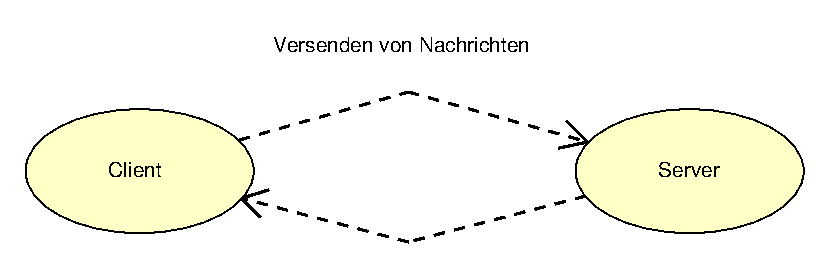
\includegraphics{images/client-server}}
	\caption{Client/Server Modell}
	\label{fig:ClientServer}
\end{figure}

Der Simulator basiert auf dem Client/Server Prinzip. Jeder Simulation besteht in der Regel aus einen teilnehmenden Client und einen Server, die miteinander \"{u}ber Nachrichten kommunizieren (Abbildung \ref{fig:ClientServer}). Bei komplexen Simulationen k\"{o}nnen auch mehrere Clients und/oder Server mitwirken. In der Regel empfangen Server nur Nachrichten, die von Clients verschickt wurden und virce versa.

\subsubsection{Prozesse und deren Rollen}

Ein verteiltes System wird anhand von Prozessen simuliert. Jeder Prozess nimmt hierbei eine oder mehrere Rollen ein. Beispielsweise kann ein Prozess die Rolle eines Clients einnehmen und ein weiterer Prozess die Rolle eines Servers. Ein Prozess kann auch Client und Server gleichzeitig sein. Es ist auch m\"{o}glich, dass ein Prozess die Rollen mehrerer Server und Clients aufeinmal einnimmt. Ob das sinnvoll ist h\"{a}ngt vom Szenario ab. Um einen Prozess zu kennzeichnen besitzt jeder Prozess eine \textbf{eindeutige} Prozess-Identifikationsnummer (PID).

\subsubsection{Nachrichten}

Damit das Client/Server Modell angewandt werden kann, m\"{u}ssen Nachrichten verschickt werden k\"{o}nnen. Eine Nachricht kann von einem Client- oder Serverprozess verschickt werden und kann beliebig viele Empf\"{a}nger haben. Der Inhalt einer Nachricht h\"{a}ngt vom verwendeten Protokoll ab. Was unter einem Protokoll zu verstehen ist, wird sp\"{a}ter behandelt. Um eine Nachricht zu kennzeichnen besitzt jede Nachricht eine \textbf{eindeutige} Nachrichten-Identifikationsnummer (NID).

\subsubsection{Lokale und globale Uhren}

In einer Simulation gibt es \textbf{genau eine} globale Uhr. Sie stellt die aktuelle und \textbf{immer korrekte} Zeit dar. Eine globale Uhr geht nie falsch.

Zudem besitzt jeder beteiligter Prozess eine eigene lokale Uhr. Sie stellt die aktuelle, jedoch nicht zwangsm\"{a}�ig global-korrekte, Zeit des jeweiligen Prozesses dar. Wenn die Prozesszeit nicht global-korrekt ist (nicht der globalen Zeit gleicht), dann wurde die Prozessuhr entweder im Laufe einer Simulation neugesetzt, oder sie geht wegen einer Uhrabweichung falsch. Die Uhrabweichung gibt an, um welchen Faktor die Uhr falsch geht. Wenn eine lokale Uhr nicht neugesetzt wird und auch keine Uhrabweichung hat, dann gleicht ihre Zeit die der globalen Uhr. 

\subsubsection{Ereignisse}

Eine Simulation besteht aus der Hintereinanderausf\"{u}hrung von endlich vielen Ereignissen. Beispielsweise kann es ein Ereignis geben, welches einen Prozess eine Nachricht verschicken- oder den Prozess selbst abst\"{u}rzen l\"{a}�t. Jedes Ereignis tritt zu einem bestimmten Zeitpunkt ein. Wenn es zeitgleiche Ereignisse gibt, so werden sie in Wirklichkeit ebenso hintereinander ausgef\"{u}hrt, erscheinen aber in der Simulation als ob sie parallel ausgef\"{u}hrt w\"{u}rden. Dieser Umstand ist auf die Implementierung des Simulators zur\"{u}ckzuf\"{u}hren, worauf sp\"{a}ter noch genauer eingegangen wird. Dem Benutzer des Simulators st\"{o}rt dies jedoch nicht, da Ereignisse aus seiner Sicht parallel ausgef\"{u}hrt werden k\"{o}nnen.

\begin{figure}[htbp]
	\centering
	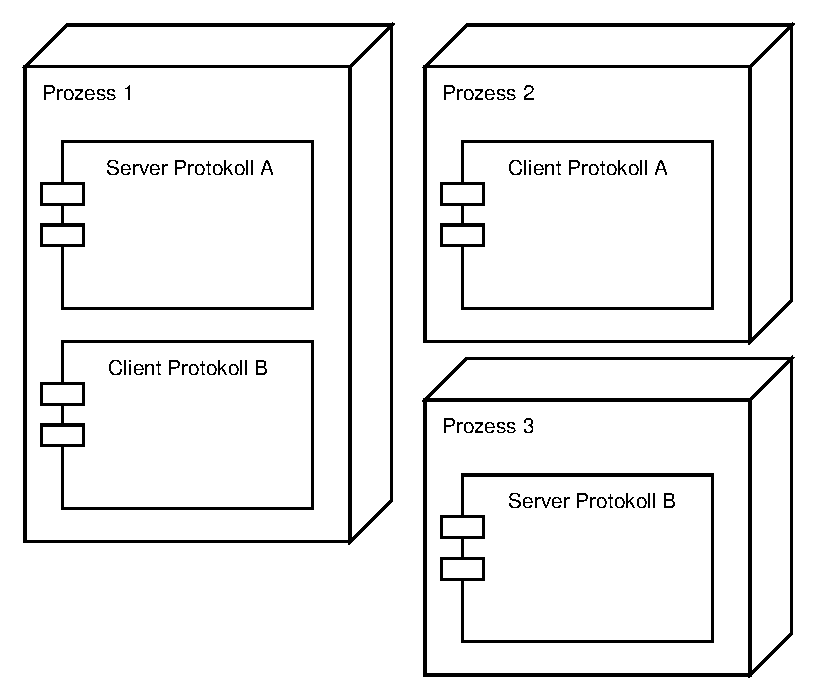
\includegraphics{images/client-server-protokolle}
	\caption{Client/Server Protokolle}
	\label{fig:ClientServerProtokolle}
\end{figure}


\subsubsection{Protokolle}

Eine Simulation besteht auch aus der Anwendung von Protokollen. Es wurde bereits erw\"{a}hnt, dass ein Prozess die Rollen von Servern und/oder Clients annehmen kann. Bei jeder Server- und Clientrolle muss zus\"{a}tzlich das dazugeh\"{o}rige Protokoll spezifiziert werden. Ein Protokoll definiert, wie ein Client und ein Server Nachrichten verschickt und wie bei Ankunft einer Nachricht reagiert wird. Ein Protokoll legt auch fest, welche Daten in einer Nachricht enthalten sind. Ein Prozess verarbeitet eine empfangene Nachricht nur, wenn er das jeweilige Protokoll versteht.

In Abbildung \ref{fig:ClientServerProtokolle} sind 3 Prozesse dargestellt. Prozess 1 unterst\"{u}tzt serverseitig das Protokoll ``A'' und clientseitig das Protokoll ``B''. Prozess 2 unterst\"{u}tzt clientseitig das Protokoll ``A'' und Prozess 3 serverseitig das Protokoll ``B''. D.h., Prozess 1 kann mit Prozess 2 via Protokoll ``A'' und mit Prozess 3 via Protokoll ``B'' kommunizieren. Die Prozesse 2 und 3 sind zueinander inkompatibel und k\"{o}nnen voneinander erhaltene Nachrichten nicht verarbeiten.

In der Regel k\"{o}nnen Clients nicht mit Clients und Server nicht mit Server kommunizieren. Je nach verwendetem Protokoll kann dies jedoch variieren. Alle vom Simulator verf\"{u}gbaren Protokolle werden sp\"{a}ter genauer behandelt.
